% !TEX TS-program = pdflatex
%%%%%%%%%%%%%%%%%%%%%%%%%%%%%%%%%%%%%%%%%%%%%%%%%%%%%%%%%%%%%%%
%
%     filename  = "YourName-Dissertation.tex",
%     version   = "1.6.5",
%     date      = "2019/07/10",
%     authors   = "Gary L. Gray,
%     copyright = "Gary L. Gray",
%     address   = "Engineering Science and Mechanics,
%                  212 Earth & Engineering Sciences Bldg.,
%                  Penn State University,
%                  University Park, PA 16802,
%                  USA",
%     telephone = "814-863-1778",
%     email     = "gray@psu.edu",
%
%%%%%%%%%%%%%%%%%%%%%%%%%%%%%%%%%%%%%%%%%%%%%%%%%%%%%%%%%%%%%%%
% Change History:
% The change history can be found in the accompanying document
% entitled "YourName-Dissertation Template Change History.md".
%%%%%%%%%%%%%%%%%%%%%%%%%%%%%%%%%%%%%%%%%%%%%%%%%%%%%%%%%%%%%%%
%
% This is a template file to help get you started using the
% psuthesis.cls for theses and dissertations at Penn State
% University. You will, of course, need to put the
% psuthesis.cls file someplace that LaTeX will find it.
%
% I have set up a directory structure that I find to be clean
% and convenient. You can readjust it to suit your tastes. In
% fact, the structure used by our students is even a little
% more involved and commands are defined to point to the
% various directories.
%
% This document has been set up to be typeset using pdflatex.
% About the only thing you will need to change if typesetting
% using latex is the \DeclareGraphicsExtensions command.
%
% The psuthesis document class uses the same options as the
% book class. In addition, it requires that you have the
% ifthen, calc, setspace, and tocloft packages.
%
% The first additional option specifies the degree type. You
% can choose from:
%	Ph.D. using class option <phd>
%	M.S. using class option <ms>
%	M.Eng. using class option <meng>
%	M.A. using class option <ma>
%	B.S. using class option <bs>
%	B.A. using class option <ba>
%	Honors from the Schreyer Honors College <schreyer>
%
% The second additional option inlinechaptertoc determines
% the formatting of the Chapter entries in the Table of
% Contents. The default sets them as two-line entries (try it).
% If you want them as one-line entries, issue the
% inlinechaptertoc option.
%
% The class option schreyer should be used for theses
% submitted to the Schreyer Honors College.
%
% The class option esc should be used by all Engineering Science
% students.
%
% The option option twoha should be used if you are earning
% interdisciplanary honors and thus have two honors advisors.
%
% The class option ``secondthesissupervisor'' should be used
% for baccalaureate honors degrees if you have a second
% Thesis Supervisor.
%
% The vita is only included with the phd option and it is
% placed at the end of the thesis. The permissions page is only
% included with the ms, meng, and ma options.
%%%%%%%%%%%%%%%%%%%%%%%%%%%%%%%%%%%%%%%%%%%%%%%%%%%%%%%%%%%%%%%
% Only one of the following lines should be used at a time.
% Doctoral students.
%\documentclass[phd,12pt]{psuthesis}
% Masters students
%\documentclass[ms,12pt]{psuthesis}
% Bachelors students in the Schreyer Honors College.
\documentclass[bs,schreyer,12pt]{psuthesis}
% Bachelors students in the Schreyer Honors College & Engineering Science.
%\documentclass[bs,schreyer,esc,twoha,12pt]{psuthesis}
% Bachelors students in Engineering Science.
%\documentclass[bs,esc,12pt]{psuthesis}

\usepackage[T1]{fontenc}
\usepackage{lmodern}
\usepackage{textcomp}
\usepackage{microtype}

%%%%%%%%%%%%%%%%%%%%%%%%%%%
% Packages I like to use. %
%%%%%%%%%%%%%%%%%%%%%%%%%%%
\usepackage{amsmath}
\usepackage{amssymb}
%\usepackage{amsthm}
%\usepackage{exscale}
%\usepackage[mathscr]{eucal}
%\usepackage{bm}
\usepackage{subfigure}
\usepackage{eqlist} % Makes for a nice list of symbols.
\usepackage[nosepfour,warning,np,debug,autolanguage]{numprint}
\usepackage{acro}
\usepackage{booktabs}
\usepackage[final]{graphicx}
\usepackage[dvipsnames]{color}
\DeclareGraphicsExtensions{.pdf, .jpg}

\usepackage{url}

% http://www.tex.ac.uk/cgi-bin/texfaq2html?label=citesort
\usepackage{cite}

\usepackage{titlesec}

%%%%%%%%%%%%%%%%%%%%%%%%%%%%%%%
% Use of the hyperref package %
%%%%%%%%%%%%%%%%%%%%%%%%%%%%%%%
%
% This is optional and is included only for those students
% who want to use it.
%
% To the hyperref package, uncomment the following line:
%\usepackage{hyperref}
%
% Note that you should also uncomment the following line:
%\renewcommand{\theHchapter}{\thepart.\thechapter}
%
% to work around some a problem hyperref has with the fact
% the psuthesis class has unnumbered pages after which page
% counters are reset.

% Set the baselinestretch using the setspace package.
% The LaTeX Companion claims that a \baselinestretch of
% 1.24 gives one-and-a-half line spacing, which is allowed
% by the PSU thesis office. As of October 18, 2013, the Graduate
% School states ``The text of an eTD may be single-, double- or
% one- and-a-half-spaced.'' Go nuts!
\setstretch{1.24}


%%%%%%%%%%%%%%%%%%%%%%%%%%%%%%%%%%%%
% SPECIAL SYMBOLS AND NEW COMMANDS %
%%%%%%%%%%%%%%%%%%%%%%%%%%%%%%%%%%%%
% Place user-defined commands below.

% Define the \acro command.
\makeatletter
\newif\ifFirstPar       \FirstParfalse
\def\smc{\sc}
\def\ninepoint{\small}
\DeclareRobustCommand\SMC{%
  \ifx\@currsize\normalsize\small\else
   \ifx\@currsize\small\footnotesize\else
    \ifx\@currsize\footnotesize\scriptsize\else
     \ifx\@currsize\large\normalsize\else
      \ifx\@currsize\Large\large\else
       \ifx\@currsize\LARGE\Large\else
        \ifx\@currsize\scriptsize\tiny\else
         \ifx\@currsize\tiny\tiny\else
          \ifx\@currsize\huge\LARGE\else
           \ifx\@currsize\Huge\huge\else
            \small\SMC@unknown@warning
 \fi\fi\fi\fi\fi\fi\fi\fi\fi\fi
}
\newcommand\SMC@unknown@warning{\TBWarning{\string\SMC: unrecognised
    text font size command -- using \string\small}}
\newcommand\textSMC[1]{{\SMC #1}}
\newcommand\acro[1]{\textSMC{#1}\@}

\makeatother

% command for vectors
\newcommand{\bv}[1]{\ensuremath{\vec{#1}}}
% command for unit vectors
\newcommand{\uv}[2][blank]{%
\ifthenelse{\equal{#1}{blank}}%
{\ensuremath{\hat{u}_{#2}}}%
{}%
%
\ifthenelse{\equal{#1}{.}}%
{\ensuremath{\dot{\hat{u}}_{#2}}}%
{}%
%
\ifthenelse{\equal{#1}{'}}%
{\ensuremath{\hat{u}'_{#2}}}%
{}%
}
\newcommand{\ui}{\ensuremath{\hat{\imath}}}
\newcommand{\uj}{\ensuremath{\hat{\jmath}}}
\newcommand{\uk}{\ensuremath{\hat{k}}}



%%%%%%%%%%%%%%%%%%%%%%%%%%%%%%%%%%%%%%%%%
% Renewed Float Parameters              %
% (Makes floats fit better on the page) %
%%%%%%%%%%%%%%%%%%%%%%%%%%%%%%%%%%%%%%%%%
\renewcommand{\floatpagefraction}{0.85}
\renewcommand{\topfraction}      {0.85}
\renewcommand{\bottomfraction}   {0.85}
\renewcommand{\textfraction}     {0.15}

% ----------------------------------------------------------- %

%%%%%%%%%%%%%%%%
% FRONT-MATTER %
%%%%%%%%%%%%%%%%
% Title
\title{Dynamics of Fish}

% Author and Department
\author{Nicholas A. Evich}
\dept{Department of Mechanical Engineering}
% the degree will be conferred on this date
\degreedate{December 2020}
% year of your copyright
\copyrightyear{2013}

% This command is used for students submitting a thesis to the
% Schreyer Honors College and for students in Engineering Science.
% The argument of this command should contain every after the word
% ``requirements'' that appears on the title page. This provides the
% needed flexibility for all the degree types.
\bachelorsdegreeinfo{for a baccalaureate degree \\ in Mechanical Engineering \\ with honors in Mechanical Engineering}

% This is the document type. For example, this could also be:
%	Comprehensive Document
%	Thesis Proposal
\documenttype{Thesis}
%\documenttype{Dissertation}
%\documenttype{Comprehensive Document}


% This will generally be The Graduate School, though you can
% put anything in here to suit your needs.
\submittedto{The Graduate School}

% This is the college to which you are submitting the
% thesis/dissertation.
\collegesubmittedto{College of Engineering}


%%%%%%%%%%%%%%%%%%
% Signatory Page %
%%%%%%%%%%%%%%%%%%
% You can have up to 7 committee members, i.e., one advisor
% and up to 6 readers.
%
% Begin by specifying the number of readers.
\numberofreaders{4}

% For baccalaureate honors degrees, enter the name of your
% honors advisor below.
\honorsadvisor{Honors P. Advisor}
{Associate Professor of Engineering Science and Mechanics}
\honorsadvisortwo{Honors P. Advisor, Jr.}
{Professor of Engineering Science and Mechanics}

% For baccalaureate honors degrees, if you have a second
% Thesis Supervisor, enter his or her name below.
\secondthesissupervisor{Second T. Supervisor}

% For baccalaureate honors degrees, certain departments
% (e.g., Engineering Science and Mechanics) require the
% signature of the department head. In that case, enter the
% name and title of your department head below.
\escdepthead{Department Q. Head}
\escdeptheadtitle{P. B. Breneman Chair and Professor 
of Engineering Science and Mechanics
}

% Input reader information below. The optional argument, which
% comes first, goes on the second line before the name.
\advisor[Thesis Advisor][Chair of Committee]
		{Joseph H. Blow}
		{Professor of SomeThing}

\readerone[Optional Title Here]
			{Reader Name}
			{Professor of SomeThing}

\readertwo[Optional Title Here]
			{Reader Name}
			{Professor of SomeThing}

\readerthree[Optional Title Here]
			{Reader Name}
			{Professor of SomeThing}

\readerfour[Optional Title Here]
			{Reader Name}
			{Professor of SomeThing}

\readerfive[Optional Title Here]
			{Reader Name}
			{Professor of SomeThing}

% Format the Chapter headings using the titlesec package.
% You can format section headings and the like here too.
\definecolor{gray75}{gray}{0.75}
\newcommand{\hsp}{\hspace{15pt}}
\titleformat{\chapter}[display]{\fontsize{30}{30}\selectfont\bfseries\sffamily}{Chapter \thechapter\hsp\textcolor{gray75}{\raisebox{3pt}{|}}}{0pt}{}{}

\titleformat{\section}[block]{\Large\bfseries\sffamily}{\thesection}{12pt}{}{}
\titleformat{\subsection}[block]{\large\bfseries\sffamily}{\thesubsection}{12pt}{}{}


% Makes use of LaTeX's include facility. Add as many chapters
% and appendices as you like.
\includeonly{%
Chapter-1/Chapter-1,%
Chapter-2/Chapter-2,%
Chapter-3/Chapter-3,%
Chapter-4/Chapter-4,%
Chapter-5/Chapter-5,%
Appendix-A/Appendix-A,%
Appendix-B/Appendix-B,%
Appendix-C/Appendix-C,%
Appendix-D/Appendix-D,%
Appendix-E/Appendix-E%
}

\usepackage{listings}
%%%%%%%%%%%%%%%%%
% THE BEGINNING %
%%%%%%%%%%%%%%%%%
\begin{document}
\pagestyle{fancy}
\fancyhead[L,C,R]{}
\fancyfoot[L,R]{}
\fancyfoot[C]{\thepage}
\renewcommand{\headrulewidth}{0pt}
\renewcommand{\footrulewidth}{0pt}
%%%%%%%%%%%%%%%%%%%%%%%%
% Preliminary Material %
%%%%%%%%%%%%%%%%%%%%%%%%
% This command is needed to properly set up the frontmatter.
\frontmatter

%%%%%%%%%%%%%%%%%%%%%%%%%%%%%%%%%%%%%%%%%%%%%%%%%%%%%%%%%%%%%%
% IMPORTANT
%
% The following commands allow you to include all the
% frontmatter in your thesis. If you don't need one or more of
% these items, you can comment it out. Most of these items are
% actually required by the Grad School -- see the Thesis Guide
% for details regarding what is and what is not required for
% your particular degree.
%%%%%%%%%%%%%%%%%%%%%%%%%%%%%%%%%%%%%%%%%%%%%%%%%%%%%%%%%%%%%%
% !!! DO NOT CHANGE THE SEQUENCE OF THESE ITEMS !!!
%%%%%%%%%%%%%%%%%%%%%%%%%%%%%%%%%%%%%%%%%%%%%%%%%%%%%%%%%%%%%%

% Generates the title page based on info you have provided
% above.
\psutitlepage

% Generates the committee page -- this is bound with your
% thesis. If this is an baccalaureate honors thesis, then
% comment out this line.
\psucommitteepage

% Generates the abstract. The argument should point to the
% file containing your abstract. 
\thesisabstract{SupplementaryMaterial/Abstract}

% Generates the Table of Contents
\thesistableofcontents

% Generates the List of Figures
\begin{singlespace}
\renewcommand{\listfigurename}{\sffamily\Huge List of Figures}
\setlength{\cftparskip}{\baselineskip}
\addcontentsline{toc}{chapter}{List of Figures}
%\fancypagestyle{plain}{%
%\fancyhf{} % clear all header and footer fields
%\fancyfoot[C]{\thepage}} % except the center
\listoffigures
\end{singlespace}
\clearpage

% Generates the List of Tables
\begin{singlespace}
\renewcommand{\listtablename}{\sffamily\Huge List of Tables}
\setlength{\cftparskip}{\baselineskip}
\addcontentsline{toc}{chapter}{List of Tables}
\listoftables
\end{singlespace}
\clearpage

% Generates the List of Symbols. The argument should point to
% the file containing your List of Symbols. 
\thesislistofsymbols{SupplementaryMaterial/ListOfSymbols}

% Generates the Acknowledgments. The argument should point to
% the file containing your Acknowledgments. 
\thesisacknowledgments{SupplementaryMaterial/Acknowledgments}

% Generates the Epigraph/Dedication. The first argument should
% point to the file containing your Epigraph/Dedication and
% the second argument should be the title of this page. 
%\thesisdedication{SupplementaryMaterial/Dedication}{Dedication}



%%%%%%%%%%%%%%%%%%%%%%%%%%%%%%%%%%%%%%%%%%%%%%%%%%%%%%
% This command is needed to get the main part of the %
% document going.                                    %
%%%%%%%%%%%%%%%%%%%%%%%%%%%%%%%%%%%%%%%%%%%%%%%%%%%%%%
\thesismainmatter

%%%%%%%%%%%%%%%%%%%%%%%%%%%%%%%%%%%%%%%%%%%%%%%%%%
% This is an AMS-LaTeX command to allow breaking %
% of displayed equations across pages. Note the  %
% closing the "}" just before the bibliography.  %
%%%%%%%%%%%%%%%%%%%%%%%%%%%%%%%%%%%%%%%%%%%%%%%%%%
\allowdisplaybreaks{
%\pagestyle{fancy}
%\fancyhead{}
%
%%%%%%%%%%%%%%%%%%%%%%
% THE ACTUAL CONTENT %
%%%%%%%%%%%%%%%%%%%%%%
% Chapters
% !TEX root = ../YourName-Dissertation.tex

\chapter{Literature Review} \label{chapter1:introduction}

\section{Homogeneous Equilibrium Model}
	\subsection{Brief outline of two-phase flows}
		\noindent Refer readers to Appendix A if they need it
	\subsection{Talk about HEM at length}
\section{Typical two-phase flow situations}
	\noindent Compare and contrast each application type in a clever way. For example, nuclear reactors and electronics are both expensive, but only electronics are feasible to change current cooling techniques. HVAC and Electronics are both feasible to change, but only advanced electronics justify the costs of optimizing and additively manufacturing designs. Possibly make a Venn diagram in which one side is "Feasible to Change" (politics) and the other side is "Justifiable Cost of Change" (economics)
	\subsection{Nuclear Reactors}
	\subsection{Heating and Ventilation Systems}
	\subsection{Advanced Electronics}
	\noindent Make it clear that electronics are the most suitable application for design tools, this necessitates some understanding of what I am trying to do (which I have not yet covered in this outline
\section{Current optimization methods}
	\subsection{Overview of engineering design tools}
		\noindent Advantages and disadvantages
	\subsection{Heat Sinks}
		\noindent Reference the Dede Paper(s)
	\subsection{Single-phase flows}
		\noindent Turbomachinery (Kirsch and Thole Paper)
	\subsection{Genetic Algorithms for other applications}
	\subsection {Nick Larimer's and my previous work}
		\noindent Stress the simplicity of these models, show a figure and some results

\section{Thesis goals and outlines}
	\begin{enumerate}
		\item Genetic Algorithms
		\item Make an actual design tool
		\item Applied to advanced electronics	
		\item One dimensional single channel design optimization
		\item Simple test cases representative of what might be seen and what might be useful in the cooling of advanced electronics
		\item Water cooled (maybe try to use other coolants if possible)
	\end{enumerate}


%\section{This is a Section}
%After discussing the overall structure, let's throw in a table.
%
%\subsection{A Table}
%Units are essential to any quantifiable measure. Newton's second law in scalar form, $F = ma$, provides for the formulation of a consistent and unambiguous system of units.  We will use both \acro{U.S.} Customary units and \acro{SI} units (International System\footnote{\acro{SI} has been adopted as the abbreviation for the French \emph{Le Syst\`{e}me International d'Unit\'{e}s}.}) as shown in Table~\ref{Ch1-table: US Customary and SI Unit Systems}. This is a url \url{https://psu.instructure.com/courses/1929919}.
%%%%%
%\begin{table}[ht]
%\caption{\label{Ch1-table: US Customary and SI Unit Systems}\acro{U.S.} Customary and \acro{SI} unit systems.}
%\begin{minipage}{\textwidth}
%\centering
%\renewcommand{\footnoterule}{\vspace{-7pt}\rule{0pt}{0pt}}
%\renewcommand{\arraystretch}{1.2}
%\begin{tabular}{l l l}
%\toprule
%& \multicolumn{2}{c}{\textbf{System of units}}\\
%\cmidrule{2-3}
%\multicolumn{1}{l}{\textbf{Base dimension}} & \emph{\acro{U.S.} Customary} & \emph{\acro{SI}} \\ \midrule
%%%
%\qquad force & pound $(\text{lb})$ & newton\footnote{derived unit} $(\text{N})
%\equiv \np[kg\text{-}m/\text{s}^{\text{2}}]{\mbox{}}$ \\
%%%
%%\panel{l}{mass} & \panel{l}{$\text{slug}^{\textit{a}} \equiv \text{lb}\cdot\text{s}^2/\text{ft}$} & \panel{l}{kilogram (kg)} \\
%\qquad mass & $\text{slug}^{\textit{a}} \equiv \np[lb\text{-}s^2/ft]{\mbox{}}$ & kilogram $(\text{kg})$ \\
%%%
%\qquad length & foot $(\text{ft})$ & meter $(\text{m})$ \\
%%%
%\qquad time & second $(\text{s})$ & second $(\text{s})$ \\ \bottomrule
%\end{tabular}
%\end{minipage}
%\end{table}
%%%%%
%
%
%\subsection{This is a Subsection}
%
%We hold these truths to be self-evident, that all men are created equal,  that they are endowed by their Creator with certain unalienable Rights,  that among these are Life, Liberty and the pursuit of Happiness. --That to secure these  rights, Governments are instituted among Men, deriving their just powers  from the consent of the governed, --That whenever any Form of Government  becomes destructive of these ends, it is the Right of the People to alter  or to abolish it, and to institute new Government, laying its foundation on  such principles and organizing its powers in such form, as to them shall  seem most likely to effect their Safety and Happiness. Prudence, indeed, will dictate that Governments long established should not  be changed for light and transient causes; and accordingly all experience  hath shewn, that mankind are more disposed to suffer, while evils are  sufferable, than to right themselves by abolishing the forms to which they  are accustomed.\cite{BhattacharyaJames-1999-A-Theory-of-Thi-0,RimrottJanabi-Sharifi-1992-A-Torque-Free-F-0,DaviesMoon-1993-3-D-Spatial-Cha-0,Tonkin-1980-A-Basic-Attitud-0,Matsumoto-1984-A-Chaotic-Attra-0,MacKay-1988-A-Criterion-for-0,FreundNix-1996-A-Critical-Thic-0,MarsdenHolmes-1979-A-Horseshoe-in--0,Koiller-1984-A-Mechanical-Sy-0,TsiotrasLonguski-1995-A-New-Parameter-0,ShimadaNagashima-1979-A-Numerical-App-0,HsuLee-1971-A-Stability-Stu-0,Muller-PfeifferKranenburg-1992-A-Two-Dimension-0,HashinShtrikman-1963-A-Variational-A-0,Junkins-1997-Adventures-on-t-0}
%%%%
%\begin{figure}%[htb]
%    \centering
%    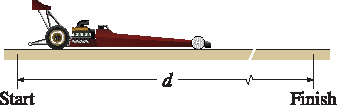
\includegraphics[scale=1.5]{Chapter-1/Figures/dragster}
%    \caption{This is a figure with a caption in a floating \texttt{figure} environment.}
%    \label{Ch1-figure: dragster}
%\end{figure}
%%%%
%
%
%\subsection{Some Equations}
%The \acro{FBD} of the box as it tips over the corner is shown at the bottom right, where we have chosen to use polar coordinates for writing the Newton-Euler equations. The Newton-Euler equations corresponding to this \acro{FBD} are
%%%
%\begin{alignat}{2}
%\label{eq: Sum Fx}
%&\sum F_{r}\!: \quad & N - mg \cos\theta &= m a_{Gr}, \\
%\label{eq: Sum Fy}
%&\sum F_{\theta}\!: \quad & mg \sin\theta - F &= m a_{G\theta}, \\
%\label{eq: Sum MG}
%&\sum M_{G}\!: \quad & F \frac{h}{2} &= I_{G} \alpha,
%\end{alignat}
%%%
%where $I_G = \frac{1}{12}m \left( h^2 + h^2 \right) = \frac{1}{6} m h^2$. Now writing the acceleration of $G$ in polar coordinates, we have
%\[
%\bv{a}_G = \left( \ddot{r} - r \dot{\theta}^2 \right) \uv{r} + \left( r \ddot{\theta} + 2 \dot{r} \dot{\theta} \right) \uv{\theta} = - \frac{h}{2} \dot{\theta}^2 \,\uv{r} + \frac{h}{2} \ddot{\theta} \,\uv{\theta},
%\]
%where we have used the fact that the distance from $A$ to $G$ is $r = h/2$ and the fact that $r$ is a constant. Substituting the acceleration components into Eqs.~\eqref{eq: Sum Fx} and~\eqref{eq: Sum Fy}, we obtain
%%%
%\begin{align}
%\label{eq: Sum Fx w/ KE}
%N - mg \cos\theta &= -m \frac{h}{2} \dot{\theta}^2, \\
%\label{eq: Sum Fy w/ KE}
%mg \sin\theta - F &= m \frac{h}{2} \ddot{\theta}.
%\end{align}
%%%
%Solving Eq.~\eqref{eq: Sum Fy w/ KE} for $F$ and substituting it into Eq.~\eqref{eq: Sum MG} and the solving for $\ddot{\theta}$, we obtain
%%%
%\begin{equation}
%\label{eq: angular accel}
%\frac{h}{2} \left( mg \sin\theta - m \frac{h}{2} \ddot{\theta} \right) = \frac{1}{6} m h^2 \ddot{\theta}
%\quad \Rightarrow \quad
%\ddot{\theta} = \frac{6g}{5h} \sin\theta.
%\end{equation}
%%%
%This expression can be substituted into Eq.~\eqref{eq: Sum Fy w/ KE} to obtain $F$ as a function of $\theta$ as
%%%
%\begin{equation}
%\label{eq: F(theta)}
%F = mg \sin\theta - m \frac{h}{2} \left( \frac{6g}{5h} \sin\theta \right) = \frac{2}{5} mg \sin\theta.
%\end{equation}
%%%
%Equation~\eqref{eq: Sum Fx w/ KE} tells us that to find $N$ as a function of $\theta$, we need to find $\dot{\theta}$ as a function of $\theta$. This can be done either by applying the work-energy principle or by integrating the expression for $\ddot{\theta}$ in Eq.~\eqref{eq: angular accel}---we will do the latter.
%
%Invoking the chain rule in Eq.~\eqref{eq: angular accel} and integrating, we obtain
%%%
%\begin{multline}
%\label{eq: integrate ang accel}
%\ddot{\theta} = \dot{\theta} \frac{d\dot{\theta}}{d\theta} = \frac{6g}{5h} \sin\theta
%\quad \Rightarrow \quad
%\int_0^{\dot{\theta}} \dot{\theta} \, d\dot{\theta} = \frac{6g}{5h} \int_0^\theta \sin\theta \,d\theta \\
%\Rightarrow \quad
%\frac{\dot{\theta}^2}{2} = -\frac{6g}{5h} \cos\theta \biggr|_0^\theta = \frac{6g}{5h} \left( 1 - \cos\theta \right)
%\quad \Rightarrow \quad
%\dot{\theta}^2 = \frac{12g}{5h} \left( 1 - \cos\theta \right).
%\end{multline}
%%%
%Substituting the expression for $\dot{\theta}^2$ in  Eq.~\eqref{eq: integrate ang accel} into Eq.~\eqref{eq: Sum Fx w/ KE} and then solving for $N$, we obtain
%%%
%\begin{equation}
%\label{eq: N(theta)}
%N = mg \cos\theta - m \frac{h}{2} \left[ \frac{12g}{5h} \left( 1 - \cos\theta \right) \right] = \frac{1}{5} mg \left( 11 \cos\theta - 6 \right).
%\end{equation}
%%%
%
%Now, the box will start to slip on the corner when $F = \mu_s N$. Using the expressions for $F$ and $N$ as functions of $\theta$ in Eqs.~\eqref{eq: F(theta)} and~\eqref{eq: N(theta)} in this force law, we obtain
%%%
%\begin{multline}
%\label{eq: theta eqn}
%\frac{2}{5} mg \sin\theta = \frac{\mu_s}{5} m g \left( 11\cos\theta - 6 \right)
%\quad \Rightarrow \quad
%2\sin\theta = \mu_s \left( 11\cos\theta - 6 \right) \\
%\Rightarrow \quad \frac{2}{\mu_s} \sin\theta = 11 \cos\theta - 6
%\quad \Rightarrow \quad
%\frac{2}{\mu_s} \sin\theta = 11 \cos\theta - 6 \\
%\Rightarrow \quad \frac{2}{11} \left( \frac{1}{\mu_s} \sin\theta + 3 \right) = \cos\theta.
%\end{multline}
%%%
%To solve the last of Eq.~\eqref{eq: theta eqn}, we let $\cos\theta = \sqrt{1 - \sin^2\theta}$, square both sides, and then rearrange to obtain a quadratic equation in $\sin\theta$ as follows
%%%
%\begin{multline}
%\frac{4}{121} \left( \frac{1}{\mu_s} \sin\theta + 3 \right)^{\!2} = 1 - \sin^2\theta
%\quad \Rightarrow \quad
%\frac{4}{121} \left( \frac{1}{\mu_s^2} \sin^2\theta + \frac{6}{\mu_s} \sin\theta + 9 \right) = 1 - \sin^2\theta \\
%\Rightarrow \quad
%\left( \frac{4}{121\mu_s^2} + 1 \right) \sin^2\theta + \frac{24}{121\mu_s} \sin\theta - \left( \frac{36}{121} - 1 \right) = 0 \\
%\Rightarrow \quad
%\left( 4 + 121\mu_s^2 \right) \sin^2\theta + 24 \mu_s \sin\theta - 85 \mu_s^2 = 0.
%\end{multline}
%%%
%Applying the quadratic formula, we obtain
%%%
%\begin{align*}
%\sin\theta &=
%\frac{
%-24\mu_s \pm \sqrt{ (24\mu_s)^2 - 4 \left(4 + 121\mu_s^2\right)\left(-85\mu_s^2\right) }
%}
%{
%2 \left( 4 + 121\mu_s^2 \right)
%} \\
%&=
%\frac{
%-24\mu_s \pm \sqrt{ 484\mu_s^2 \left(4 + 85\mu_s^2\right) }
%}
%{
%2 \left( 4 + 121\mu_s^2 \right)
%} \\
%&=
%\frac{
%-24\mu_s \pm 22\mu_s \sqrt{ 4 + 85\mu_s^2 }
%}
%{
%2 \left( 4 + 121\mu_s^2 \right)
%} \\
%&=
%\frac{
%\mu_s \left( -12 \pm 11 \sqrt{ 4 + 85\mu_s^2 } \right)
%}
%{
%4 + 121\mu_s^2
%}.
%\end{align*}
%%%
%Therefore, the angle at which the box slips is
%\[
%\theta = \sin^{-1} \left[ \frac{
%\mu_s \left( -12 \pm 11 \sqrt{ 4 + 85\mu_s^2 } \right)
%}
%{
%4 + 121\mu_s^2
%} \right].
%\]
%For example, for $\mu_s = 1/3$, the two angles are $\theta = 32.78^\circ$ for the plus root and $\theta = -90^\circ$ for the minus root. Obviously, the physically meaningful result is the angle corresponding to the plus root.
%
%
%\subsubsection{This is a Subsubsection}
%\label{Ch1 subsection on SMAs}
%
%We hold these truths subsubsection~\ref{Ch1 subsection on SMAs} to be self-evident, that all men are created equal,  that they are endowed by their Creator with certain unalienable Rights,  that among these are Life, Liberty and the pursuit of Happiness. That to secure these  rights, Governments are instituted among Men, deriving their just powers  from the consent of the governed, That whenever any Form of Government  becomes destructive of these ends, it is the Right of the People to alter  or to abolish it, and to institute new Government, laying its foundation on  such principles and organizing its powers in such form, as to them shall  seem most likely to effect their Safety and Happiness. Prudence, indeed, will dictate that Governments long established should not  be changed for light and transient causes; and accordingly all experience  hath shewn, that mankind are more disposed to suffer, while evils are  sufferable, than to right themselves by abolishing the forms to which they  are accustomed~\cite{SmithDavenport-1988-A-Perturbation--0,Ketema-1992-A-Physical-Inte-0,GraesserCozzarelli-1994-A-Proposed-Thre-0,RichardsonMitchell-1999-A-Simplified-Va-0,MitchellRichardson-1999-A-Simplified-Va-0,Parks-1967-A-Stability-Cri-0}.
%%%%
%\begin{figure}[bt]
%    \centering
%    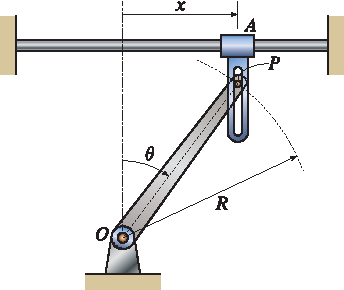
\includegraphics[width=3in]{Chapter-1/Figures/mechanism}
%    \caption{We hold these truths to be self-evident, that all men are created equal,  that they are endowed by their Creator with certain unalienable Rights,  that among these are Life, Liberty and the pursuit of Happiness.}
%    \label{Ch1-figure: mechanism}
%\end{figure}
%%%%
%Check out Fig.~\ref{Ch1-figure: mechanism}!
%
%
%\section{More Declaration}
%
%We hold these truths to be self-evident, that all men are created equal,  that they are endowed by their Creator with certain unalienable Rights,  that among these are Life, Liberty and the pursuit of Happiness. That to secure these  rights, Governments are instituted among Men, deriving their just powers  from the consent of the governed, That whenever any Form of Government  becomes destructive of these ends, it is the Right of the People to alter  or to abolish it, and to institute new Government, laying its foundation on  such principles and organizing its powers in such form, as to them shall  seem most likely to effect their Safety and Happiness. Prudence, indeed, will dictate that Governments long established should not  be changed for light and transient causes; and accordingly all experience  hath shewn, that mankind are more disposed to suffer, while evils are  sufferable, than to right themselves by abolishing the forms to which they  are accustomed.
%%%%
%\begin{figure}[htb]
%    \centering
%    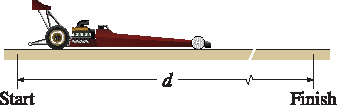
\includegraphics[scale=1.5]{Chapter-1/Figures/dragster}
%    \caption{We hold these truths to be self-evident, that all men are created equal,  that they are endowed by their Creator with certain unalienable Rights,  that among these are Life, Liberty and the pursuit of Happiness.}
%    \label{ChX-figure: FigureLabel3}
%\end{figure}
%%%%
%But when a long train of abuses and usurpations, pursuing invariably the same  Object evinces a design to reduce them under absolute Despotism, it is their  right, it is their duty, to throw off such Government, and to provide new Guards for their future security. --Such has been the patient sufferance of these Colonies; and such is now the  necessity which constrains them to alter their former Systems of Government.  The history of the present King of Great Britain [George III] is a history  of repeated injuries and usurpations, all having in direct object the  establishment of an absolute Tyranny over these States. To prove this, let Facts be submitted to a candid world.
%
%We hold these truths to be self-evident, that all men are created equal,  that they are endowed by their Creator with certain unalienable Rights,  that among these are Life, Liberty and the pursuit of Happiness. That to secure these  rights, Governments are instituted among Men, deriving their just powers  from the consent of the governed, That whenever any Form of Government  becomes destructive of these ends, it is the Right of the People to alter  or to abolish it, and to institute new Government, laying its foundation on  such principles and organizing its powers in such form, as to them shall  seem most likely to effect their Safety and Happiness. Prudence, indeed, will dictate that Governments long established should not  be changed for light and transient causes; and accordingly all experience  hath shewn, that mankind are more disposed to suffer, while evils are  sufferable, than to right themselves by abolishing the forms to which they  are accustomed.
%%%%
%\begin{figure}[htb]
%    \centering
%    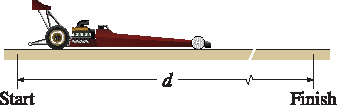
\includegraphics[scale=1.5]{Chapter-1/Figures/dragster}
%    \caption{We hold these truths to be self-evident, that all men are created equal,  that they are endowed by their Creator with certain unalienable Rights,  that among these are Life, Liberty and the pursuit of Happiness.}
%    \label{ChX-figure: FigureLabel4}
%\end{figure}
%%%%
%But when a long train of abuses and usurpations, pursuing invariably the same  Object evinces a design to reduce them under absolute Despotism, it is their  right, it is their duty, to throw off such Government, and to provide new Guards for their future security. --Such has been the patient sufferance of these Colonies; and such is now the  necessity which constrains them to alter their former Systems of Government.  The history of the present King of Great Britain [George III] is a history  of repeated injuries and usurpations, all having in direct object the  establishment of an absolute Tyranny over these States. To prove this, let Facts be submitted to a candid world.
%
%We hold these truths to be self-evident, that all men are created equal,  that they are endowed by their Creator with certain unalienable Rights,  that among these are Life, Liberty and the pursuit of Happiness. That to secure these  rights, Governments are instituted among Men, deriving their just powers  from the consent of the governed, That whenever any Form of Government  becomes destructive of these ends, it is the Right of the People to alter  or to abolish it, and to institute new Government, laying its foundation on  such principles and organizing its powers in such form, as to them shall  seem most likely to effect their Safety and Happiness. Prudence, indeed, will dictate that Governments long established should not  be changed for light and transient causes; and accordingly all experience  hath shewn, that mankind are more disposed to suffer, while evils are  sufferable, than to right themselves by abolishing the forms to which they  are accustomed.
%%%%
%\begin{figure}[htb]
%    \centering
%    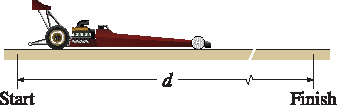
\includegraphics[scale=1.5]{Chapter-1/Figures/dragster}
%    \caption{We hold these truths to be self-evident, that all men are created equal,  that they are endowed by their Creator with certain unalienable Rights,  that among these are Life, Liberty and the pursuit of Happiness.}
%    \label{ChX-figure: FigureLabel5}
%\end{figure}
%%%%
%But when a long train of abuses and usurpations, pursuing invariably the same  Object evinces a design to reduce them under absolute Despotism, it is their  right, it is their duty, to throw off such Government, and to provide new Guards for their future security. --Such has been the patient sufferance of these Colonies; and such is now the  necessity which constrains them to alter their former Systems of Government.  The history of the present King of Great Britain [George III] is a history  of repeated injuries and usurpations, all having in direct object the  establishment of an absolute Tyranny over these States. To prove this, let Facts be submitted to a candid world.
%
%We hold these truths to be self-evident, that all men are created equal,  that they are endowed by their Creator with certain unalienable Rights,  that among these are Life, Liberty and the pursuit of Happiness. That to secure these  rights, Governments are instituted among Men, deriving their just powers  from the consent of the governed, That whenever any Form of Government  becomes destructive of these ends, it is the Right of the People to alter  or to abolish it, and to institute new Government, laying its foundation on  such principles and organizing its powers in such form, as to them shall  seem most likely to effect their Safety and Happiness. Prudence, indeed, will dictate that Governments long established should not  be changed for light and transient causes; and accordingly all experience  hath shewn, that mankind are more disposed to suffer, while evils are  sufferable, than to right themselves by abolishing the forms to which they  are accustomed.
%%%%
%\begin{figure}[htb]
%    \centering
%    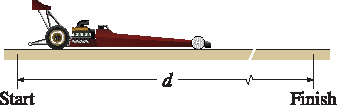
\includegraphics[scale=1.5]{Chapter-1/Figures/dragster}
%    \caption{We hold these truths to be self-evident, that all men are created equal,  that they are endowed by their Creator with certain unalienable Rights,  that among these are Life, Liberty and the pursuit of Happiness.}
%    \label{ChX-figure: FigureLabel6}
%\end{figure}
%%%%
%But when a long train of abuses and usurpations, pursuing invariably the same  Object evinces a design to reduce them under absolute Despotism, it is their  right, it is their duty, to throw off such Government, and to provide new Guards for their future security. --Such has been the patient sufferance of these Colonies; and such is now the  necessity which constrains them to alter their former Systems of Government.  The history of the present King of Great Britain [George III] is a history  of repeated injuries and usurpations, all having in direct object the  establishment of an absolute Tyranny over these States. To prove this, let Facts be submitted to a candid world.
%
%We hold these truths to be self-evident, that all men are created equal,  that they are endowed by their Creator with certain unalienable Rights,  that among these are Life, Liberty and the pursuit of Happiness. That to secure these  rights, Governments are instituted among Men, deriving their just powers  from the consent of the governed, That whenever any Form of Government  becomes destructive of these ends, it is the Right of the People to alter  or to abolish it, and to institute new Government, laying its foundation on  such principles and organizing its powers in such form, as to them shall  seem most likely to effect their Safety and Happiness. Prudence, indeed, will dictate that Governments long established should not  be changed for light and transient causes; and accordingly all experience  hath shewn, that mankind are more disposed to suffer, while evils are  sufferable, than to right themselves by abolishing the forms to which they  are accustomed.
%%%%
%\begin{figure}[htb]
%    \centering
%    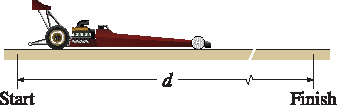
\includegraphics[scale=1.5]{Chapter-1/Figures/dragster}
%    \caption{We hold these truths to be self-evident, that all men are created equal,  that they are endowed by their Creator with certain unalienable Rights,  that among these are Life, Liberty and the pursuit of Happiness.}
%    \label{ChX-figure: FigureLabel7}
%\end{figure}
%%%%
%But when a long train of abuses and usurpations, pursuing invariably the same  Object evinces a design to reduce them under absolute Despotism, it is their  right, it is their duty, to throw off such Government, and to provide new Guards for their future security. --Such has been the patient sufferance of these Colonies; and such is now the  necessity which constrains them to alter their former Systems of Government.  The history of the present King of Great Britain [George III] is a history  of repeated injuries and usurpations, all having in direct object the  establishment of an absolute Tyranny over these States. To prove this, let Facts be submitted to a candid world.
%
%We hold these truths to be self-evident, that all men are created equal,  that they are endowed by their Creator with certain unalienable Rights,  that among these are Life, Liberty and the pursuit of Happiness. That to secure these  rights, Governments are instituted among Men, deriving their just powers  from the consent of the governed, That whenever any Form of Government  becomes destructive of these ends, it is the Right of the People to alter  or to abolish it, and to institute new Government, laying its foundation on  such principles and organizing its powers in such form, as to them shall  seem most likely to effect their Safety and Happiness. Prudence, indeed, will dictate that Governments long established should not  be changed for light and transient causes; and accordingly all experience  hath shewn, that mankind are more disposed to suffer, while evils are  sufferable, than to right themselves by abolishing the forms to which they  are accustomed.
%%%%
%\begin{figure}[htb]
%    \centering
%    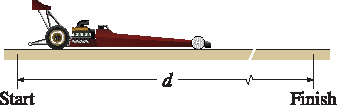
\includegraphics[scale=1.5]{Chapter-1/Figures/dragster}
%    \caption{We hold these truths to be self-evident, that all men are created equal,  that they are endowed by their Creator with certain unalienable Rights,  that among these are Life, Liberty and the pursuit of Happiness.}
%    \label{ChX-figure: FigureLabel8}
%\end{figure}
%%%%
%But when a long train of abuses and usurpations, pursuing invariably the same  Object evinces a design to reduce them under absolute Despotism, it is their  right, it is their duty, to throw off such Government, and to provide new Guards for their future security. --Such has been the patient sufferance of these Colonies; and such is now the  necessity which constrains them to alter their former Systems of Government.  The history of the present King of Great Britain [George III] is a history  of repeated injuries and usurpations, all having in direct object the  establishment of an absolute Tyranny over these States. To prove this, let Facts be submitted to a candid world.
%
%We hold these truths to be self-evident, that all men are created equal,  that they are endowed by their Creator with certain unalienable Rights,  that among these are Life, Liberty and the pursuit of Happiness. That to secure these  rights, Governments are instituted among Men, deriving their just powers  from the consent of the governed, That whenever any Form of Government  becomes destructive of these ends, it is the Right of the People to alter  or to abolish it, and to institute new Government, laying its foundation on  such principles and organizing its powers in such form, as to them shall  seem most likely to effect their Safety and Happiness. Prudence, indeed, will dictate that Governments long established should not  be changed for light and transient causes; and accordingly all experience  hath shewn, that mankind are more disposed to suffer, while evils are  sufferable, than to right themselves by abolishing the forms to which they  are accustomed.
%%%%
%\begin{figure}[htb]
%    \centering
%    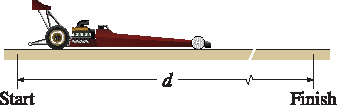
\includegraphics[scale=1.5]{Chapter-1/Figures/dragster}
%    \caption{We hold these truths to be self-evident, that all men are created equal,  that they are endowed by their Creator with certain unalienable Rights,  that among these are Life, Liberty and the pursuit of Happiness.}
%    \label{ChX-figure: FigureLabel9}
%\end{figure}
%%%%
%But when a long train of abuses and usurpations, pursuing invariably the same  Object evinces a design to reduce them under absolute Despotism, it is their  right, it is their duty, to throw off such Government, and to provide new Guards for their future security. --Such has been the patient sufferance of these Colonies; and such is now the  necessity which constrains them to alter their former Systems of Government.  The history of the present King of Great Britain [George III] is a history  of repeated injuries and usurpations, all having in direct object the  establishment of an absolute Tyranny over these States. To prove this, let Facts be submitted to a candid world.
%
%We hold these truths to be self-evident, that all men are created equal,  that they are endowed by their Creator with certain unalienable Rights,  that among these are Life, Liberty and the pursuit of Happiness. That to secure these  rights, Governments are instituted among Men, deriving their just powers  from the consent of the governed, That whenever any Form of Government  becomes destructive of these ends, it is the Right of the People to alter  or to abolish it, and to institute new Government, laying its foundation on  such principles and organizing its powers in such form, as to them shall  seem most likely to effect their Safety and Happiness. Prudence, indeed, will dictate that Governments long established should not  be changed for light and transient causes; and accordingly all experience  hath shewn, that mankind are more disposed to suffer, while evils are  sufferable, than to right themselves by abolishing the forms to which they  are accustomed.
%%%%
%\begin{figure}[htb]
%    \centering
%    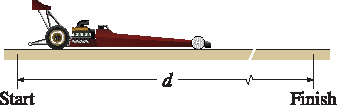
\includegraphics[scale=1.5]{Chapter-1/Figures/dragster}
%    \caption{We hold these truths to be self-evident, that all men are created equal,  that they are endowed by their Creator with certain unalienable Rights,  that among these are Life, Liberty and the pursuit of Happiness.}
%    \label{ChX-figure: FigureLabel10}
%\end{figure}
%%%%
%But when a long train of abuses and usurpations, pursuing invariably the same  Object evinces a design to reduce them under absolute Despotism, it is their  right, it is their duty, to throw off such Government, and to provide new Guards for their future security. --Such has been the patient sufferance of these Colonies; and such is now the  necessity which constrains them to alter their former Systems of Government.  The history of the present King of Great Britain [George III] is a history  of repeated injuries and usurpations, all having in direct object the  establishment of an absolute Tyranny over these States. To prove this, let Facts be submitted to a candid world.
%
%We hold these truths to be self-evident, that all men are created equal,  that they are endowed by their Creator with certain unalienable Rights,  that among these are Life, Liberty and the pursuit of Happiness. That to secure these  rights, Governments are instituted among Men, deriving their just powers  from the consent of the governed, That whenever any Form of Government  becomes destructive of these ends, it is the Right of the People to alter  or to abolish it, and to institute new Government, laying its foundation on  such principles and organizing its powers in such form, as to them shall  seem most likely to effect their Safety and Happiness. Prudence, indeed, will dictate that Governments long established should not  be changed for light and transient causes; and accordingly all experience  hath shewn, that mankind are more disposed to suffer, while evils are  sufferable, than to right themselves by abolishing the forms to which they  are accustomed.
%%%%
%\begin{figure}[htb]
%    \centering
%    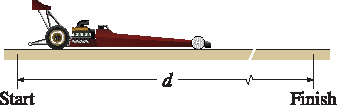
\includegraphics[scale=1.5]{Chapter-1/Figures/dragster}
%    \caption{We hold these truths to be self-evident, that all men are created equal,  that they are endowed by their Creator with certain unalienable Rights,  that among these are Life, Liberty and the pursuit of Happiness.}
%    \label{ChX-figure: FigureLabel3}
%\end{figure}
%%%%
%But when a long train of abuses and usurpations, pursuing invariably the same  Object evinces a design to reduce them under absolute Despotism, it is their  right, it is their duty, to throw off such Government, and to provide new Guards for their future security. --Such has been the patient sufferance of these Colonies; and such is now the  necessity which constrains them to alter their former Systems of Government.  The history of the present King of Great Britain [George III] is a history  of repeated injuries and usurpations, all having in direct object the  establishment of an absolute Tyranny over these States. To prove this, let Facts be submitted to a candid world.
%% !TEX root = ../YourName-Dissertation.tex

\chapter{Title of the Second Chapter}

\section{Introduction}
When in the Course of human events, it becomes necessary for one people  to dissolve the political bands which have connected them with another,  and to assume among the powers of the earth, the separate and equal station  to which the Laws of Nature and of Nature's God entitle them, a decent respect to the opinions of mankind requires that they should declare  the causes which impel them to the separation.

\section{More Declaration}

We hold these truths to be self-evident, that all men are created equal,  that they are endowed by their Creator with certain unalienable Rights,  that among these are Life, Liberty and the pursuit of Happiness. --That to secure these  rights, Governments are instituted among Men, deriving their just powers  from the consent of the governed, --That whenever any Form of Government  becomes destructive of these ends, it is the Right of the People to alter  or to abolish it, and to institute new Government, laying its foundation on  such principles and organizing its powers in such form, as to them shall  seem most likely to effect their Safety and Happiness. Prudence, indeed, will dictate that Governments long established should not  be changed for light and transient causes; and accordingly all experience  hath shewn, that mankind are more disposed to suffer, while evils are  sufferable, than to right themselves by abolishing the forms to which they  are accustomed. But when a long train of abuses and usurpations, pursuing invariably the same  Object evinces a design to reduce them under absolute Despotism, it is their  right, it is their duty, to throw off such Government, and to provide new Guards for their future security. --Such has been the patient sufferance of these Colonies; and such is now the  necessity which constrains them to alter their former Systems of Government.
%%
\begin{equation}
\label{eq: label}
x = y
\end{equation}
%%
The history of the present King of Great Britain [George III] is a history  of repeated injuries and usurpations, all having in direct object the  establishment of an absolute Tyranny over these States. To prove this, let Facts be submitted to a candid world.
%% !TEX root = ../YourName-Dissertation.tex

\chapter{Title of the Third Chapter}

\section{Introduction}
When in the Course of human events, it becomes necessary for one people  to dissolve the political bands which have connected them with another,  and to assume among the powers of the earth, the separate and equal station  to which the Laws of Nature and of Nature's God entitle them, a decent respect to the opinions of mankind requires that they should declare  the causes which impel them to the separation.

\section{More Declaration}

We hold these truths to be self-evident, that all men are created equal,  that they are endowed by their Creator with certain unalienable Rights,  that among these are Life, Liberty and the pursuit of Happiness. --That to secure these  rights, Governments are instituted among Men, deriving their just powers  from the consent of the governed, --That whenever any Form of Government  becomes destructive of these ends, it is the Right of the People to alter  or to abolish it, and to institute new Government, laying its foundation on  such principles and organizing its powers in such form, as to them shall  seem most likely to effect their Safety and Happiness. Prudence, indeed, will dictate that Governments long established should not  be changed for light and transient causes; and accordingly all experience  hath shewn, that mankind are more disposed to suffer, while evils are  sufferable, than to right themselves by abolishing the forms to which they  are accustomed. But when a long train of abuses and usurpations, pursuing invariably the same  Object evinces a design to reduce them under absolute Despotism, it is their  right, it is their duty, to throw off such Government, and to provide new Guards for their future security. --Such has been the patient sufferance of these Colonies; and such is now the  necessity which constrains them to alter their former Systems of Government.  The history of the present King of Great Britain [George III] is a history  of repeated injuries and usurpations, all having in direct object the  establishment of an absolute Tyranny over these States. To prove this, let Facts be submitted to a candid world.
%% !TEX root = ../YourName-Dissertation.tex

\chapter{Title of the Fourth Chapter}

\section{Introduction}
When in the Course of human events, it becomes necessary for one people  to dissolve the political bands which have connected them with another,  and to assume among the powers of the earth, the separate and equal station  to which the Laws of Nature and of Nature's God entitle them, a decent respect to the opinions of mankind requires that they should declare  the causes which impel them to the separation.

\section{More Declaration}

We hold these truths to be self-evident, that all men are created equal,  that they are endowed by their Creator with certain unalienable Rights,  that among these are Life, Liberty and the pursuit of Happiness. --That to secure these  rights, Governments are instituted among Men, deriving their just powers  from the consent of the governed, --That whenever any Form of Government  becomes destructive of these ends, it is the Right of the People to alter  or to abolish it, and to institute new Government, laying its foundation on  such principles and organizing its powers in such form, as to them shall  seem most likely to effect their Safety and Happiness. Prudence, indeed, will dictate that Governments long established should not  be changed for light and transient causes; and accordingly all experience  hath shewn, that mankind are more disposed to suffer, while evils are  sufferable, than to right themselves by abolishing the forms to which they  are accustomed.

\subsection{Some nonsense here}

But when a long train of abuses and usurpations, pursuing invariably the same  Object evinces a design to reduce them under absolute Despotism, it is their  right, it is their duty, to throw off such Government, and to provide new Guards for their future security. --Such has been the patient sufferance of these Colonies; and such is now the  necessity which constrains them to alter their former Systems of Government.

\subsection{Some additional nonsense here}

The history of the present King of Great Britain [George III] is a history  of repeated injuries and usurpations, all having in direct object the  establishment of an absolute Tyranny over these States. To prove this, let Facts be submitted to a candid world.
%% !TEX root = ../YourName-Dissertation.tex

\chapter{Title of the Fifth Chapter}

\section{Introduction}
When in the Course of human events, it becomes necessary for one people  to dissolve the political bands which have connected them with another,  and to assume among the powers of the earth, the separate and equal station  to which the Laws of Nature and of Nature's God entitle them, a decent respect to the opinions of mankind requires that they should declare  the causes which impel them to the separation.

\section{More Declaration}

We hold these truths to be self-evident, that all men are created equal,  that they are endowed by their Creator with certain unalienable Rights,  that among these are Life, Liberty and the pursuit of Happiness. --That to secure these  rights, Governments are instituted among Men, deriving their just powers  from the consent of the governed, --That whenever any Form of Government  becomes destructive of these ends, it is the Right of the People to alter  or to abolish it, and to institute new Government, laying its foundation on  such principles and organizing its powers in such form, as to them shall  seem most likely to effect their Safety and Happiness. Prudence, indeed, will dictate that Governments long established should not  be changed for light and transient causes; and accordingly all experience  hath shewn, that mankind are more disposed to suffer, while evils are  sufferable, than to right themselves by abolishing the forms to which they  are accustomed. But when a long train of abuses and usurpations, pursuing invariably the same  Object evinces a design to reduce them under absolute Despotism, it is their  right, it is their duty, to throw off such Government, and to provide new Guards for their future security. --Such has been the patient sufferance of these Colonies; and such is now the  necessity which constrains them to alter their former Systems of Government.  The history of the present King of Great Britain [George III] is a history  of repeated injuries and usurpations, all having in direct object the  establishment of an absolute Tyranny over these States. To prove this, let Facts be submitted to a candid world.
%%%%%%%%%%%%%%%%%%%%%%%%%%%%%%%%%%%%%%%%%%%%%%%%%%%%%%%%%%%%%%%
% Appendices
%
% Because of a quirk in LaTeX (see p. 48 of The LaTeX
% Companion, 2e), you cannot use \include along with
% \addtocontents if you want things to appear the proper
% sequence.
%%%%%%%%%%%%%%%%%%%%%%%%%%%%%%%%%%%%%%%%%%%%%%%%%%%%%%%%%%%%%%%
\appendix
\titleformat{\chapter}[display]{\fontsize{30}{30}\selectfont\bfseries\sffamily}{Appendix \thechapter\textcolor{gray75}{\raisebox{3pt}{|}}}{0pt}{}{}
% If you have a single appendix, then to prevent LaTeX from
% calling it ``Appendix A'', you should uncomment the following two
% lines that redefine the \thechapter and \thesection:
%\renewcommand\thechapter{}
%\renewcommand\thesection{\arabic{section}}
% !TEX root = ../YourName-Dissertation.tex
\Appendix{Detailed Discussion of Two-Phase Flows}

\section{Introduction}
When in the Course of human events, it becomes necessary for one people  to dissolve the political bands which have connected them with another,  and to assume among the powers of the earth, the separate and equal station  to which the Laws of Nature and of Nature's God entitle them, a decent respect to the opinions of mankind requires that they should declare  the causes which impel them to the separation.

\section{More Declaration}

We hold these truths to be self-evident, that all men are created equal,  that they are endowed by their Creator with certain unalienable Rights,  that among these are Life, Liberty and the pursuit of Happiness. --That to secure these  rights, Governments are instituted among Men, deriving their just powers  from the consent of the governed, --That whenever any Form of Government  becomes destructive of these ends, it is the Right of the People to alter  or to abolish it, and to institute new Government, laying its foundation on  such principles and organizing its powers in such form, as to them shall  seem most likely to effect their Safety and Happiness.

\subsection{Some Subsection Title Here}

Prudence, indeed, will dictate that Governments long established should not  be changed for light and transient causes; and accordingly all experience  hath shewn, that mankind are more disposed to suffer, while evils are  sufferable, than to right themselves by abolishing the forms to which they  are accustomed. But when a long train of abuses and usurpations, pursuing invariably the same  Object evinces a design to reduce them under absolute Despotism, it is their  right, it is their duty, to throw off such Government, and to provide new Guards for their future security. --Such has been the patient sufferance of these Colonies; and such is now the  necessity which constrains them to alter their former Systems of Government.  The history of the present King of Great Britain [George III] is a history  of repeated injuries and usurpations, all having in direct object the  establishment of an absolute Tyranny over these States. To prove this, let Facts be submitted to a candid world.
% !TEX root = ../YourName-Dissertation.tex
\Appendix{Title of the Second Appendix}

\section{Introduction}
When in the Course of human events, it becomes necessary for one people  to dissolve the political bands which have connected them with another,  and to assume among the powers of the earth, the separate and equal station  to which the Laws of Nature and of Nature's God entitle them, a decent respect to the opinions of mankind requires that they should declare  the causes which impel them to the separation.

\section{More Declaration}

We hold these truths to be self-evident, that all men are created equal,  that they are endowed by their Creator with certain unalienable Rights,  that among these are Life, Liberty and the pursuit of Happiness. --That to secure these  rights, Governments are instituted among Men, deriving their just powers  from the consent of the governed, --That whenever any Form of Government  becomes destructive of these ends, it is the Right of the People to alter  or to abolish it, and to institute new Government, laying its foundation on  such principles and organizing its powers in such form, as to them shall  seem most likely to effect their Safety and Happiness. Prudence, indeed, will dictate that Governments long established should not  be changed for light and transient causes; and accordingly all experience  hath shewn, that mankind are more disposed to suffer, while evils are  sufferable, than to right themselves by abolishing the forms to which they  are accustomed. But when a long train of abuses and usurpations, pursuing invariably the same  Object evinces a design to reduce them under absolute Despotism, it is their  right, it is their duty, to throw off such Government, and to provide new Guards for their future security. --Such has been the patient sufferance of these Colonies; and such is now the  necessity which constrains them to alter their former Systems of Government.  The history of the present King of Great Britain [George III] is a history  of repeated injuries and usurpations, all having in direct object the  establishment of an absolute Tyranny over these States. To prove this, let Facts be submitted to a candid world.
% !TEX root = ../YourName-Dissertation.tex
\Appendix{Title of the Third Appendix}

\section{Introduction}
When in the Course of human events, it becomes necessary for one people  to dissolve the political bands which have connected them with another,  and to assume among the powers of the earth, the separate and equal station  to which the Laws of Nature and of Nature's God entitle them, a decent respect to the opinions of mankind requires that they should declare  the causes which impel them to the separation.

\section{More Declaration}

We hold these truths to be self-evident, that all men are created equal,  that they are endowed by their Creator with certain unalienable Rights,  that among these are Life, Liberty and the pursuit of Happiness. --That to secure these  rights, Governments are instituted among Men, deriving their just powers  from the consent of the governed, --That whenever any Form of Government  becomes destructive of these ends, it is the Right of the People to alter  or to abolish it, and to institute new Government, laying its foundation on  such principles and organizing its powers in such form, as to them shall  seem most likely to effect their Safety and Happiness. Prudence, indeed, will dictate that Governments long established should not  be changed for light and transient causes; and accordingly all experience  hath shewn, that mankind are more disposed to suffer, while evils are  sufferable, than to right themselves by abolishing the forms to which they  are accustomed. But when a long train of abuses and usurpations, pursuing invariably the same  Object evinces a design to reduce them under absolute Despotism, it is their  right, it is their duty, to throw off such Government, and to provide new Guards for their future security. --Such has been the patient sufferance of these Colonies; and such is now the  necessity which constrains them to alter their former Systems of Government.  The history of the present King of Great Britain [George III] is a history  of repeated injuries and usurpations, all having in direct object the  establishment of an absolute Tyranny over these States. To prove this, let Facts be submitted to a candid world.
% !TEX root = ../YourName-Dissertation.tex
\Appendix{Title of the Fourth Appendix}

\section{Introduction}
When in the Course of human events, it becomes necessary for one people  to dissolve the political bands which have connected them with another,  and to assume among the powers of the earth, the separate and equal station  to which the Laws of Nature and of Nature's God entitle them, a decent respect to the opinions of mankind requires that they should declare  the causes which impel them to the separation.

\section{More Declaration}

We hold these truths to be self-evident, that all men are created equal,  that they are endowed by their Creator with certain unalienable Rights,  that among these are Life, Liberty and the pursuit of Happiness. --That to secure these  rights, Governments are instituted among Men, deriving their just powers  from the consent of the governed, --That whenever any Form of Government  becomes destructive of these ends, it is the Right of the People to alter  or to abolish it, and to institute new Government, laying its foundation on  such principles and organizing its powers in such form, as to them shall  seem most likely to effect their Safety and Happiness. Prudence, indeed, will dictate that Governments long established should not  be changed for light and transient causes; and accordingly all experience  hath shewn, that mankind are more disposed to suffer, while evils are  sufferable, than to right themselves by abolishing the forms to which they  are accustomed. But when a long train of abuses and usurpations, pursuing invariably the same  Object evinces a design to reduce them under absolute Despotism, it is their  right, it is their duty, to throw off such Government, and to provide new Guards for their future security. --Such has been the patient sufferance of these Colonies; and such is now the  necessity which constrains them to alter their former Systems of Government.  The history of the present King of Great Britain [George III] is a history  of repeated injuries and usurpations, all having in direct object the  establishment of an absolute Tyranny over these States. To prove this, let Facts be submitted to a candid world.
% !TEX root = ../YourName-Dissertation.tex
\Appendix{Title of the Fifth Appendix}

\section{Introduction}
When in the Course of human events, it becomes necessary for one people  to dissolve the political bands which have connected them with another,  and to assume among the powers of the earth, the separate and equal station  to which the Laws of Nature and of Nature's God entitle them, a decent respect to the opinions of mankind requires that they should declare  the causes which impel them to the separation.

\pagebreak
Some text.
{\lstset{language=Fortran}
\footnotesize
\begin{lstlisting}
      program chaos
c When a LS Fortran program has been compiled and linked into Mac
c application, all information written to the screen WRITE(6,...) or
c WRITE(*,...) appears in a standard Mac window, complete with basic
c menus.
      external fex, jac
      double precision atol, rtol, rwork, t, tout, h
      double precision ttotal, dtout
      dimension h(3), atol(3), rwork(70), iwork(23)
	  character*8 tstart, tend
      neq = 3
	  
	  call time(tstart)
	  write(6,*) "begin integration at  ", tstart
      write(6,*)
	  
c --- Read in the total initial angular momentum.  The total angular
c     momentum H is always unity due to normalization.
	  open(unit = 2, file = 'chaos.data', status = 'unknown')
      read(2,*) h(1), h(2), h(3)
	  
c --- The integration begins at t = 0 and the values are printed at
c     every tout.  tout is incremented below.  ttotal is the length
c     of the entire integration.  The number of recorded values of
c     the integration is given by npoints.
      t = 0.0d0
      tout = 0.0d0
      write(6,*) 'Duration of integration interval, i.e., tfinal?'
      read(6,*) ttotal
      write(6,*)
      write(6,*) 'Number of points for trajectory plot?'
      read(6,*) npoints
      write(6,*)
      dtout = ttotal/dfloat(npoints)
      tout = tout + dtout
	  
c --- Tolerance parameters used by lsoda.
      itol = 2
      rtol = 1.0d-9
      atol(1) = 1.0d-9
      atol(2) = 1.0d-9
      atol(3) = 1.0d-9
	  
c --- Other parameters used by lsoda.  See below.
      itask = 1
      istate = 1
      iopt = 1
      lrw = 70
      liw = 23
      jt = 1

      do 11 kount = 5,10
         rwork(kount) = 0.0d0
         iwork(kount) = 0
  11  continue
      iwork(6) = 100000
	  
	  open(unit = 3, file = 'traj.dat', disp = 'keep',
     &     status = 'unknown')
	 
c --- The actual integration begins here.  Loop on the value of iout.
      do 40 iout = 1, npoints
	  
         call lsoda(fex,neq,h,t,tout,itol,rtol,atol,itask,istate,
     &              iopt,rwork,lrw,iwork,liw,jdum,jt)
	  
c ------ Write the output to the file traj.dat.
         write(3,20) t, h(1), h(2), h(3)
  20     format(f9.1, 3e15.6)

         if (mod(tout,5000.0d0) .eq. 0.0d0) then
            write(6,*) tout
         end if
  
c ------ Check to see that things are going OK.
         if (istate .lt. 0) go to 80
		 
c ------ Set the time at which the integration is next recorded and
c        continue the do-loop.
  40     tout = tout + dtout
  
      write(6,*) 'number of steps taken: ', iwork(11)
      write(6,*) 'number of f evaluations: ', iwork(12)
      write(6,*) 'number of Jacobian evaluations: ', iwork(13)
      write(6,*) 'method order last used: ', iwork(14)
      write(6,*) 'method last used (2 = stiff): ', iwork(19)
      write(6,*) 'value of t at last method switch: ', rwork(15)
      write(6,*)
	 
	  call time(tend)
	  write(6,*) "end integration at  ", tend
      stop
	  
c --- If there is an error, given by istate < 0, write the following.
  80  write(6,90) istate
  90  format(///22h error halt.. istate =,i3)
  
      stop
      end

\end{lstlisting}
}

%%%%%%%%%%%%%%%%%%%%%%%%%%%%%%%%%%%%%%%%%%%%%%%%%%%%%%%%%%%%%%%
% ESM students need to include a Nontechnical Abstract as the %
% last appendix.                                              %
%%%%%%%%%%%%%%%%%%%%%%%%%%%%%%%%%%%%%%%%%%%%%%%%%%%%%%%%%%%%%%%
% This \include command should point to the file containing
% that abstract.
%\include{nontechnical-abstract}
%%%%%%%%%%%%%%%%%%%%%%%%%%%%%%%%%%%%%%%%%%%
} % End of the \allowdisplaybreak command %
%%%%%%%%%%%%%%%%%%%%%%%%%%%%%%%%%%%%%%%%%%%

%%%%%%%%%%%%%%%%
% BIBLIOGRAPHY %
%%%%%%%%%%%%%%%%
% You can use BibTeX or other bibliography facility for your
% bibliography. LaTeX's standard stuff is shown below. If you
% bibtex, then this section should look something like:
	\begin{singlespace}
	\bibliographystyle{GLG-bibstyle}
	\addcontentsline{toc}{chapter}{Bibliography}
	\bibliography{Biblio-Database}
	\end{singlespace}

%\begin{singlespace}
%\begin{thebibliography}{99}
%\addcontentsline{toc}{chapter}{Bibliography}
%\frenchspacing

%\bibitem{Wisdom87} J. Wisdom, ``Rotational Dynamics of Irregularly Shaped Natural Satellites,'' \emph{The Astronomical Journal}, Vol.~94, No.~5, 1987  pp. 1350--1360.

%\bibitem{G&H83} J. Guckenheimer and P. Holmes, \emph{Nonlinear Oscillations, Dynamical Systems, and Bifurcations of Vector Fields}, Springer-Verlag, New York, 1983.

%\end{thebibliography}
%\end{singlespace}

\backmatter

% Vita
\vita{SupplementaryMaterial/Vita}

\end{document}

